%
% split.tex
%
\section{Chart::Split}
\name{Chart::Split}
\file{Split.pm}
\requires{Chart::Base, GD, Carp, FileHandle}
\begin{Description} 
\class{Split} is a subclass of class \class{Chart::Base}.\\
The class \class{Split} creates a lines chart. 
Split makes always an xy-plot, which means that both axes are numeric. 
The x-axis will be split in several parts of a same interval (option 'interval' has to be set!).
These intervals will be drawn one upon the other. 
The top interval starts at the start point, 
which has to be set by the programmer (option 'start'). \\
The first passed dataset are the x coordinates. 
The following added sets are the y coordinates of the sets.\\
Split draws only positive x-coordinates.\\
The y-axis is a numbering of the intervals.\\
The Split module is useful if you have a lot of data points to plot. An example is to plot
weather or seismic data.
\end{Description}

\parindent 0pt{\large Example:} 

\begin{figure}[h]
	\begin{center}
		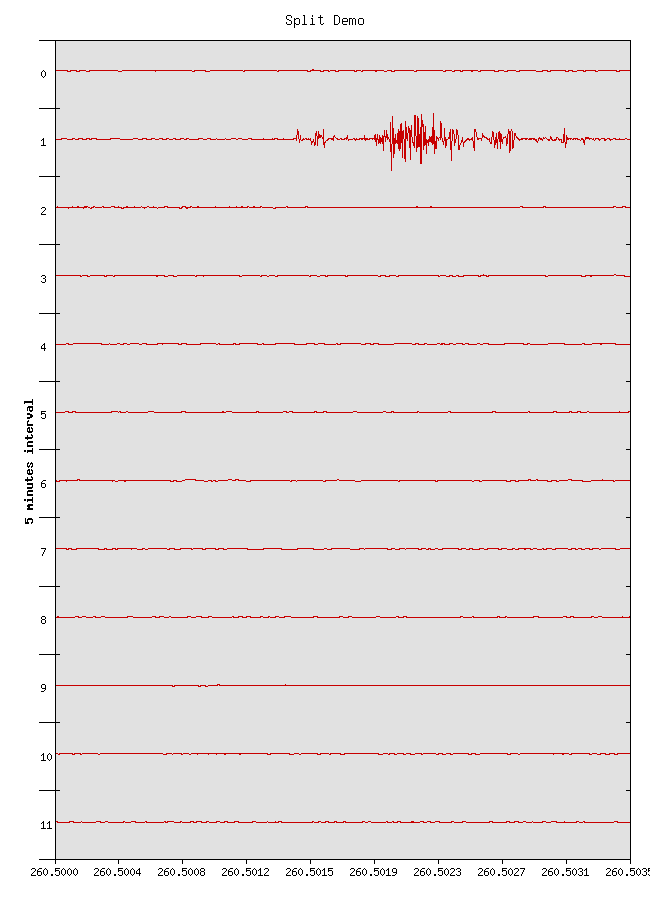
\includegraphics[width = 10cm, height =10cm]{stunde.png}
	\end{center}
	\caption{Split chart}
	\label{fig:split}
\end{figure}
\begin{verbatim}
use Chart::Split;

$g = Chart::Split->new(650 ,900);

#get the data that are in a file and push them in arrays
open( FILE , "data.dat") or die 'Can't open the data file!\n';
while (defined ($line = <FILE>) ) {
  ($x, $y,) = unpack("a11 x1 a8" , $line);
   push (@y, $y);
   push (@x, $x);
}
close (FILE);

#add the data
$g->add_dataset(@x);
$g->add_dataset(@y);

#set the options
$g->set('xy_plot' => 'true');
$g->set('legend' => 'none');
$g->set('title' => 'Split Demo');
$g->set('interval' => 1/288);
$g->set('interval_ticks' => 10);
$g->set('start' => 260.5);
$g->set('brush_size' => 1);
$g->set('precision' => 4);
$g->set('y_label' => '5 minutes interval');

#give me a nice picture
$g->png("split.png");
\end{verbatim}

\begin{Constructor} 
An instance of a split chart object can be created with the constructor \textit{new()}:
\begin{quote}
\fett{\$obj = Chart::Split->new();}\\
\fett{\$obj = Chart::Split->new(\parameter{width}, \parameter{height});}
\end{quote}

If \textit{new()} has no arguments, 
the constructor returns an image with the size 300x400 pixels. If new has two arguments 
\parameter{width} and \parameter{height}, it returns an image with the desired size.
\end{Constructor}

\Methods
All universal valid methods, see page \pageref{methods} of class
\class{Chart::Base}.\\[\parabstand]
%
\Attributes
All universal valid options, see page \pageref{options}. 
Also available, these special options:
\begin{description}
\item['start'] \emph{Required} value for a split chart. \\
               If the x coordinate of the first data point is zero, 
               you should set start to zero. 
               Sets the start value of the first interval. Defaults to undef.
               
\item['interval'] \emph{Required} value of a split chart.\\
                Sets the interval of one line to plot. Defaults to undef.
                
\item['interval\_ticks'] Sets the number of ticks for the x-axis. Defaults to 5.

\item['scale'] Every y-value of a split chart will be multiplied by that value, 
               but the scale won't be changed. This means you may overdraw certain rows! 
               Only useful if you want to give prominence to the maximal amplitudes of the data.
               Defaults to 1.
               
\item['sort'] Sorts the data ascending if set to 'true'. 
              Should be set if the added data isn't sorted. Defaults to 'false'.  
              
\item['y\_axes'] Tells chart where to place the y-axis. 
                 Valid values are 'left', 'right' and 'both'. Defaults to 'left'.
\end{description}
